\documentclass[a4paper,man,natbib,floatsintext,12pt]{apa7}

\usepackage{rotating}
\usepackage{threeparttable}
\usepackage[english]{babel} %character and hyphenation rules specific to the language you choose
%\usepackage[utf8x]{inputenc}
\usepackage{graphicx}
\usepackage{color}
\usepackage{tikz}
\usepackage{amsmath}
\usepackage{blindtext}
\usepackage{tabularx} %great for APA-style Tables
\usepackage{siunitx} % Required for good table alignmen
\sisetup{
  round-mode          = places, % Rounds numbers
  round-precision     = 2, % to 2 places
}
\usepackage{multirow}
\usepackage{booktabs}
\usepackage{wrapfig}
\usetikzlibrary{shapes,decorations,arrows,calc,arrows.meta,fit,positioning}
\tikzset{
    -Latex,auto,node distance =1 cm and 1 cm,semithick,
    latent/.style ={ellipse, draw, minimum width = 0.7 cm},
    observed/.style ={rectangle, draw},
    bidirected/.style={Latex-Latex,dashed},
    el/.style = {inner sep=2pt, align=left, sloped}
}
\newcommand{\sigFtest}[4]{\textit{F}(#1,#2) = #3, \textit{p}$<$#4}
\newcommand{\nonsigFtest}[3]{\textit{F}(#1,#2) = #3, \textit{p}$>$.05}


\title{Changes of Identification with Educational Value and Academic Prosocial Behavior among Early Adolescents and Their Relationship with Perceived Economic Inequality and Well-being}
\shorttitle{Identification with Educational Value and Prosocial Behavior}
\author{Tingyi Zhang}
\affiliation{College of William \& Mary}
\journal{PSYC672 Assignment 1}
\abstract{This study investigated changes in identification with educational value (IEV) and academic prosocial behavior (APB) among a sample of 634 early adolescents. Data were collected with a two-wave longitudinal design over seven months across consecutive school terms. It also explored whether perceived economic inequality predicts these changes, as well as links with subjective well-being (positive affect, negative affect, and life satisfaction). Latent change score models revealed that (a) IEV and APB levels, which covaried, decreased over time; (b) higher perceived economic inequality predicted greater declines in IEV; and (c) smaller decreases in IEV and APB were associated with higher subjective well-being, and the patterns of their associations with different components of well-being showed some nuances. The weaker-than-expected relationship between perceived economic inequality and changes in APB was discussed with particular attention. Findings highlight the importance of changes in students’ academic motivation and prosocial behavior and enrich understanding of how perceived economic inequality affects young adolescents’ development.}
\keywords{Perceived economic inequality, identification with educational value, academic prosocial behavior, subjective well-being, latent change score model}
\authornote{This manuscript was prepared for PSYC672. I would like to thank Professor Kieffaber for guidance on this assignment.}

\setlength{\headheight}{15pt}

%-------------- END PREAMBLE  -------------------


\begin{document}

\maketitle  %Insert my APA style title page

\section{Introduction}

Identification with educational value (IEV) and academic prosocial behavior (APB) are two important indicators of students’ academic motivation and socioemotional development, both of which have been found to predict well-being \citep{guay2018motivation, carlo2020prosocial}. However, studies suggest that IEV and APB often decline during late primary and middle school years, potentially hindering students’ positive development. Recent research also highlights the role of perceived economic inequality, a macro-level factor shaping psychological processes such as competitiveness and cooperativeness, in influencing students’ school experiences \citep{king2022inequality, sommet2023inequality}. Building on these findings, the present study asks whether perceived economic inequality predicts declines in IEV and APB among Chinese primary school students. We hypothesize that higher perceived economic inequality will be associated with greater decreases in IEV and APB over time.


\section{Method}

We conducted a two-wave longitudinal survey study to examine the role of perceived economic inequality in predicting changes in students’ identification with educational values (IEV) and academic prosocial behavior (APB). Standardized questionnaires were administered in classroom settings, and data were analyzed using latent change score models.

\subsection{Participants}
Participants were 634 students (approximately 10 years old) recruited from a primary school in northern China. Data were collected in two waves, separated by a seven-month interval. Only students with valid responses at both waves were included in the final sample.

\subsection{Materials and Procedure}
Students completed paper-and-pencil questionnaires during regular school hours. Measures included perceived economic inequality, identification with educational values (IEV), academic prosocial behavior (APB), and subjective well-being. Data were analyzed using latent change score (LCS) models in Mplus, with measurement invariance tested across waves. Model fit was evaluated using multiple indices, including RMSEA, CFI, and SRMR.

\section{Results}

Descriptive statistics and correlations among study variables are shown in Table~\ref{tab:correlations}. Overall, both identification with educational value (IEV) and academic prosocial behavior (APB) significantly declined from Time 1 to Time 2. As illustrated in the latent change score models (Figure~\ref{fig:LCM_simple}), IEV showed a significant negative change ($\beta = -0.334, p < .001$), and APB also declined ($\beta = -0.514, p < .001$). Moreover, changes in IEV and APB were positively correlated, suggesting that students who showed stronger declines in one domain tended to show stronger declines in the other.  

The full structural model (Figure~\ref{fig:LCM_full}) further indicated that perceived economic inequality (PEI) at baseline predicted greater decreases in IEV over time, but was not significantly related to changes in APB. Declines in IEV were associated with decreases in life satisfaction, while declines in APB were associated with decreases in positive affect and increases in negative affect. These findings provide partial support for our hypothesis that perceived economic inequality would predict reductions in IEV and APB, and confirm that both declines are linked with reduced well-being.  

\begin{figure}[htbp]
\centering
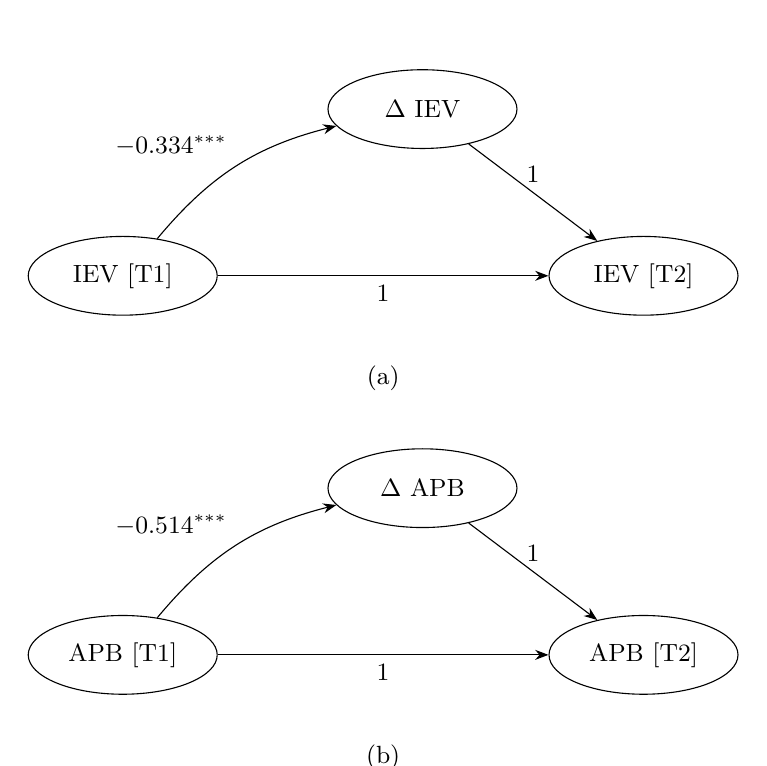
\begin{tikzpicture}[node distance=2.8cm, >=Stealth, every node/.style={font=\small}]

  \tikzstyle{state}=[ellipse, draw, minimum width=24mm, minimum height=10mm, align=center]

  \node[state]                          (IEV1)   {IEV [T1]};
  \node[state, right=4.2cm of IEV1]     (IEV2)   {IEV [T2]};
  \node[state, above right=1.4cm and 2.1cm of IEV1] (dIEV) {$\Delta$ IEV};

  \draw[->] (IEV1) -- node[below] {1} (IEV2);
  \draw[->] (dIEV) -- node[above] {1} (IEV2);
  \draw[->, bend left=18] (IEV1) to node[above left] {$-0.334^{***}$} (dIEV);

  \node at ($(IEV1)!0.5!(IEV2)+(0,-1.3)$) {(a)};

  \node[state, below=3.8cm of IEV1]          (APB1)   {APB [T1]};
  \node[state, right=4.2cm of APB1]          (APB2)   {APB [T2]};
  \node[state, above right=1.4cm and 2.1cm of APB1] (dAPB) {$\Delta$ APB};

  \draw[->] (APB1) -- node[below] {1} (APB2);
  \draw[->] (dAPB) -- node[above] {1} (APB2);
  \draw[->, bend left=18] (APB1) to node[above left] {$-0.514^{***}$} (dAPB);

  \node at ($(APB1)!0.5!(APB2)+(0,-1.3)$) {(b)};
\end{tikzpicture}
\caption{Latent change score models for IEV (a) and APB (b).}
\label{fig:LCM_simple}
\end{figure}


\begin{figure}[htbp]
\centering
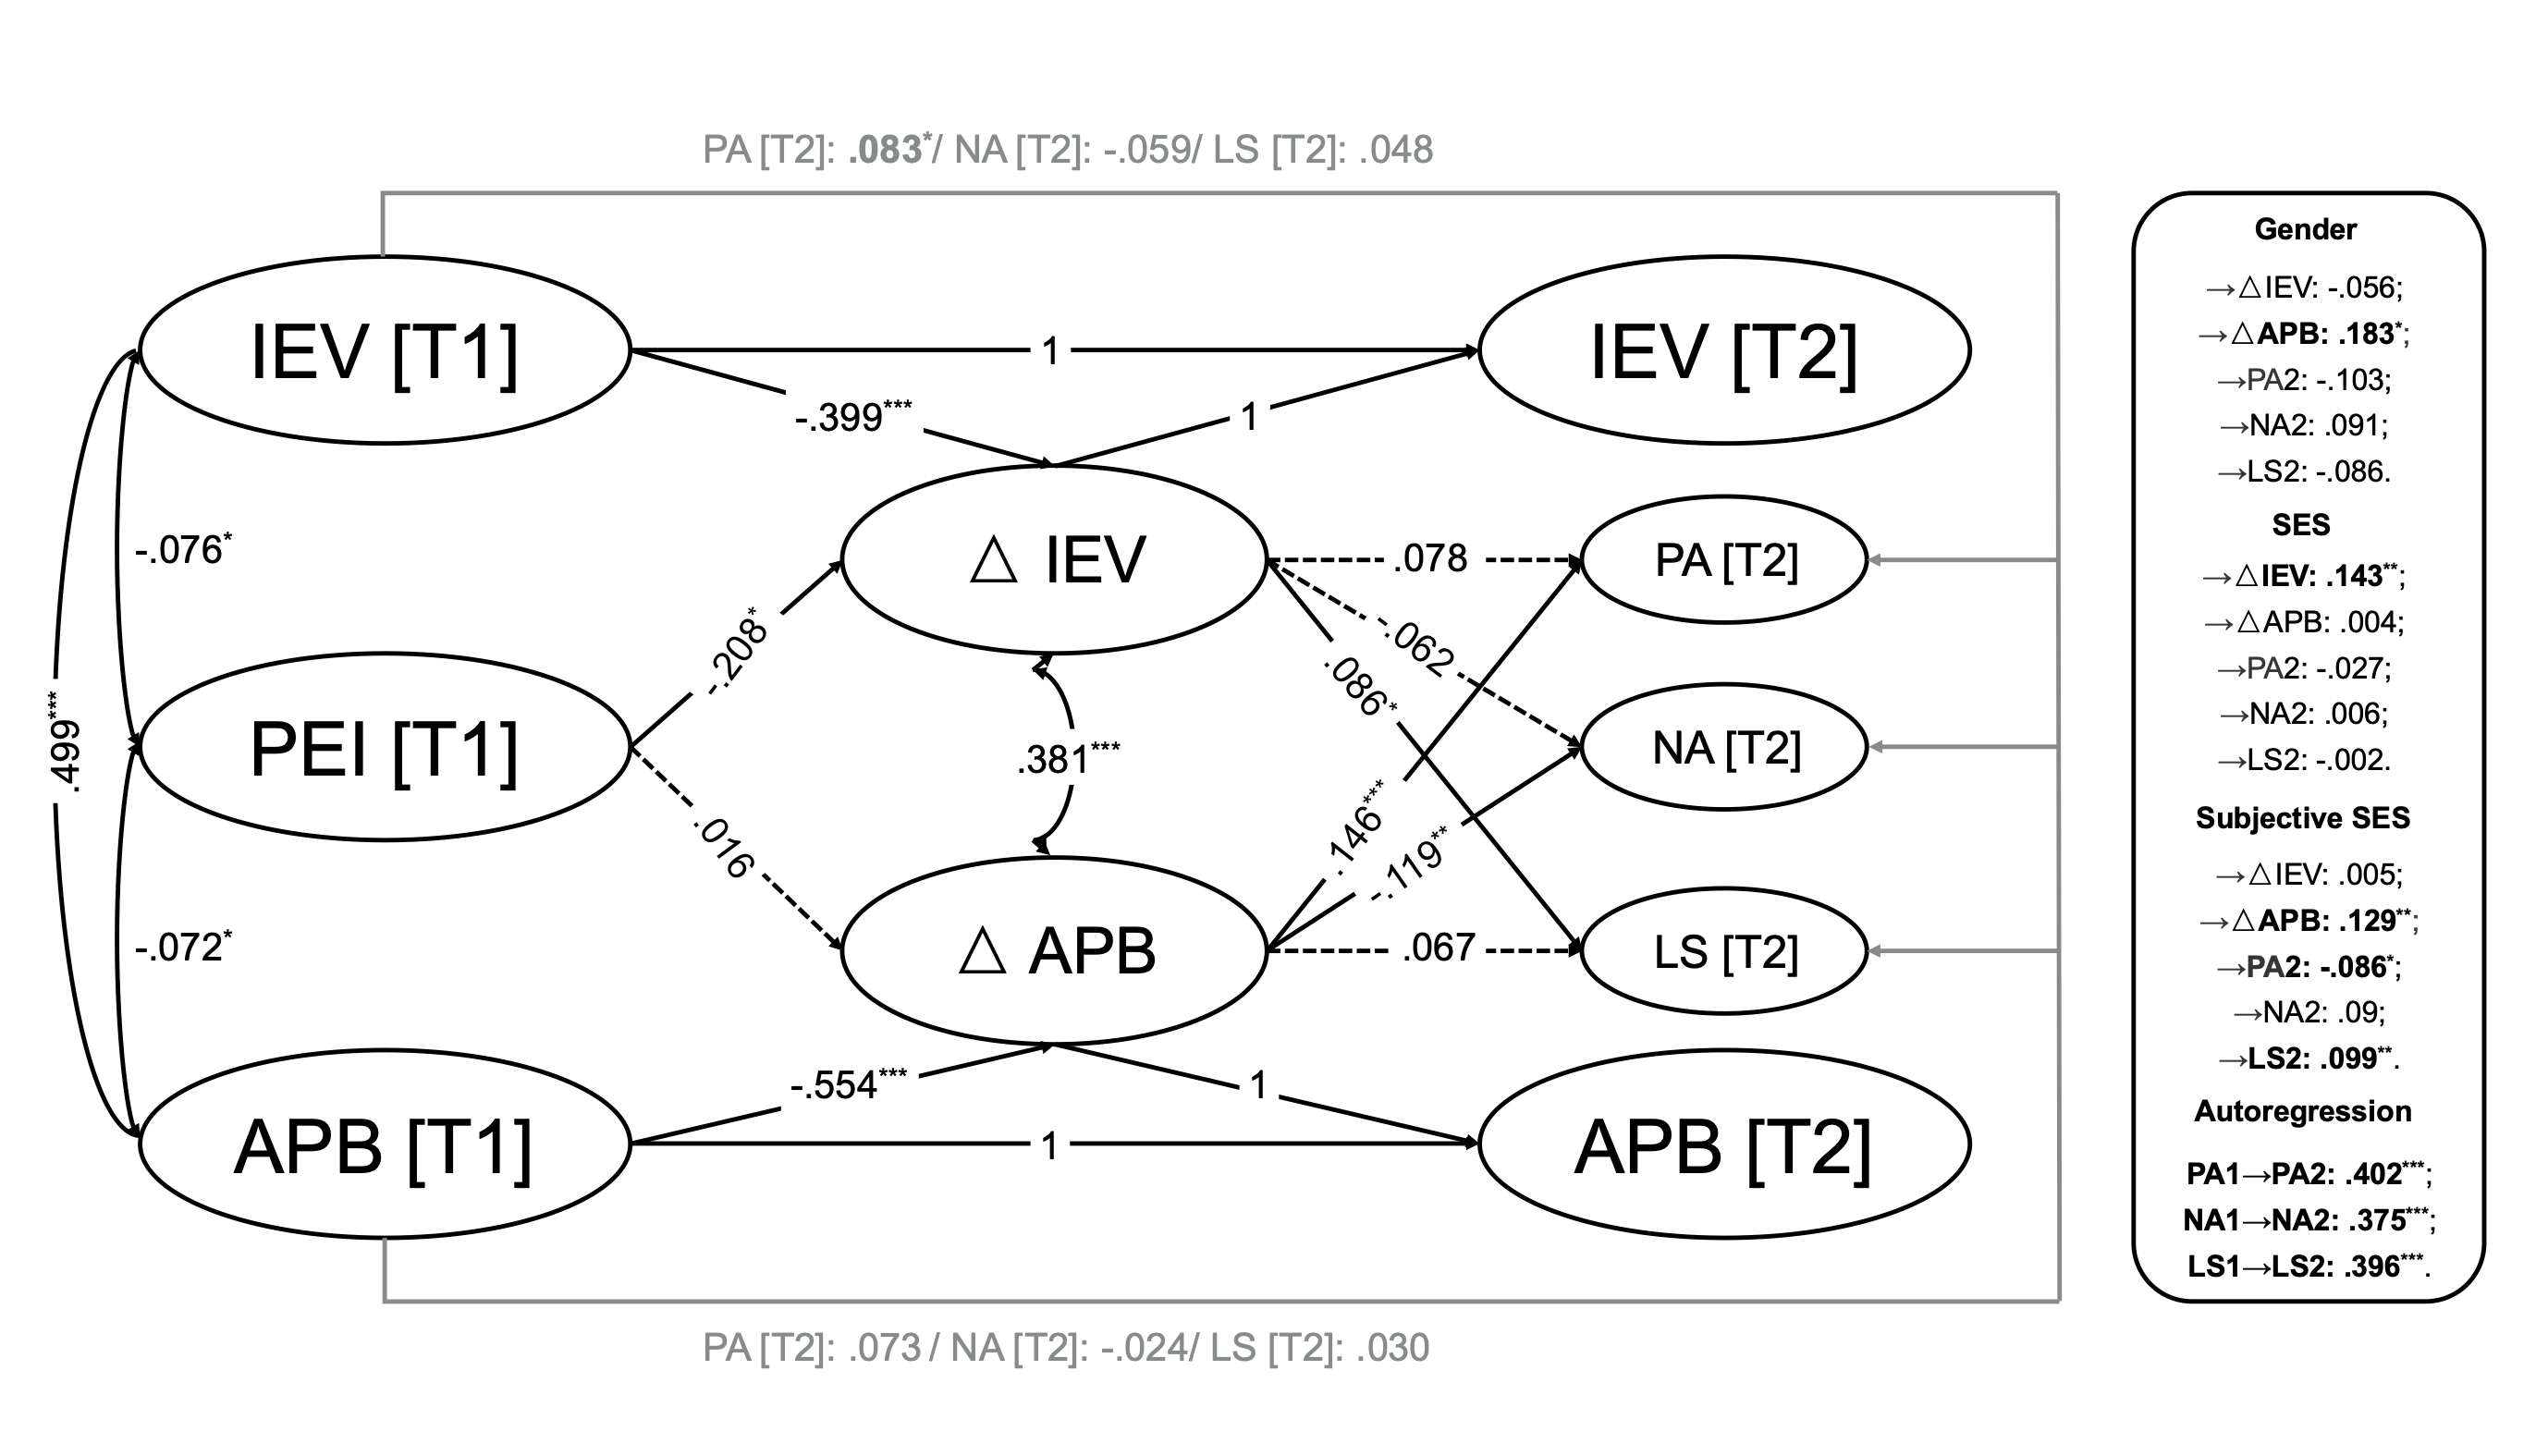
\includegraphics[width=0.9\textwidth]{20250829_Figure3.png}
\caption{Full structural model including perceived economic inequality (PEI), identification with educational value (IEV), academic prosocial behavior (APB), and well-being indicators.}
\label{fig:LCM_full}
\end{figure}

\begin{sidewaystable}[htbp]
\centering
\caption{Descriptive statistics and correlations among study variables}
\label{tab:correlations}
\begin{threeparttable}
\begin{tabular}{lcccccccccccccc}
\toprule
Variable & $M$ & $SD$ & ICC & 1 & 2 & 3 & 4 & 5 & 6 & 7 & 8 & 9 & 10 & 11 \\
\midrule
1. T1 PEI        & 2.73 & 1.494 & \textbf{.108} & -- \\
2. T1 IEV        & 5.73 & 1.245 & .018  & -.103* & -- \\
3. T2 IEV        & 5.35 & 1.476 & $<$.001 & -.143*** & .575*** & -- \\
4. T1 APB        & 5.18 & 1.643 & .015  & -.085 & .399*** & .208*** & -- \\
5. T2 APB        & 4.95 & 1.757 & .025  & -.043 & .202*** & .390*** & .511*** & -- \\
6. T1 PA         & 3.72 & 1.083 & .011  & -.179*** & .205*** & .102* & .324*** & .260*** & -- \\
7. T2 PA         & 3.65 & 1.007 & .017  & -.151** & .160** & .215*** & .161*** & .295*** & .515*** & -- \\
8. T1 NA         & 2.61 & 1.058 & .021  & .166** & -.104 & -.086 & -.014 & -.115* & -.405*** & -.330*** & -- \\
9. T2 NA         & 2.49 & .932  & .046  & .229*** & -.092 & -.216*** & .042 & -.188*** & -.316*** & -.452*** & .568*** & -- \\
10. T1 LS        & 3.34 & 1.183 & .002  & -.087 & .201*** & -.030 & .224*** & .136*** & .341*** & .282*** & -.265*** & -.092 & -- \\
11. T2 LS        & 3.36 & 1.083 & \textbf{.077} & -.109* & .116* & .158*** & .114* & .201*** & .290*** & .506*** & -.235*** & -.423*** & .484*** & -- \\
\bottomrule
\end{tabular}
\begin{tablenotes}
\footnotesize
\item \textit{Note}. $N = 634$. PEI = Perceived Economic Inequality; IEV = Identification with Educational Values; APB = Academic Prosocial Behavior; PA = Positive Affect; NA = Negative Affect; LS = Life Satisfaction. 
\item * $p < .05$. ** $p < .01$. *** $p < .001$.
\end{tablenotes}
\end{threeparttable}
\end{sidewaystable}



\section{Discussion}
Our findings suggest that early adolescents’ identification with educational value (IEV) and academic prosocial behavior (APB) both declined over time, and that perceived economic inequality predicted the decline in IEV but not APB. These results indicate that macro-level factors such as economic inequality may undermine students’ academic motivation, while APB and IEV play distinct roles in shaping adolescents’ subsequent well-being.


\bibliography{references.bib}

\end{document}
https://www.overleaf.com/project/64ef8e5b3faa92d4248ddcf9